\documentclass[11pt,reqno,a4paper]{amsart}
\usepackage{amssymb,amsmath}
\usepackage{tikz,tikz-cd}
\usetikzlibrary{calc}
\usepackage{hyperref}\hypersetup{colorlinks=true, linkcolor=purple, citecolor=blue}

\begin{document}

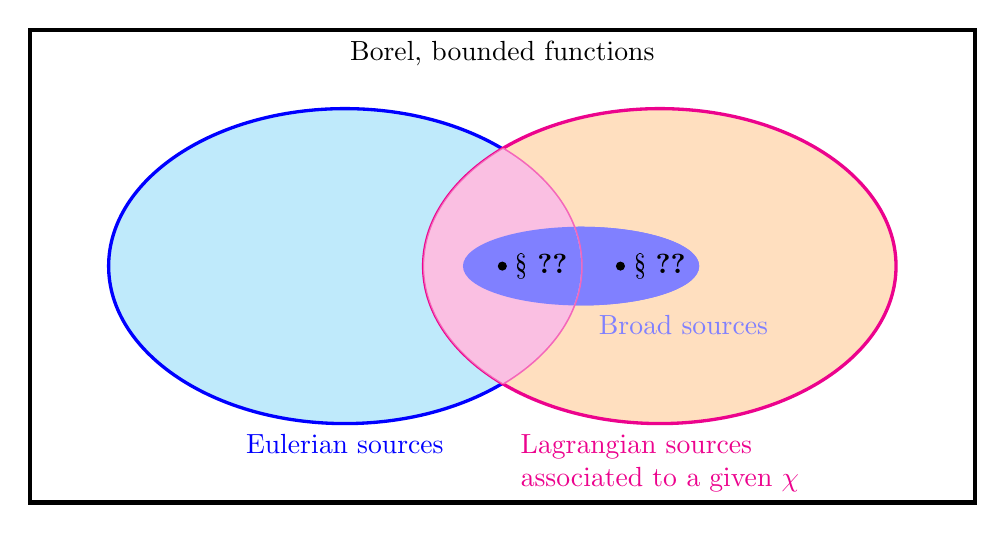
\begin{tikzpicture}
\draw[ultra thick, ->] (0,0) rectangle (12,6) 
(6,6) node[align=left, below] {Borel, bounded functions};
\filldraw[color=blue, fill=cyan!25, very thick](4,3) circle (3 and 2) (4,1) node[align=left, below] {Eulerian sources};
\filldraw[color=magenta!99, fill=orange!25, very thick](8,3) circle (3 and 2) (8,1) node[align=left, below] {Lagrangian sources\\ associated to a given $\chi$};
\fill[blue!50] (7,3) ellipse (1.5 and 0.5) (8.3,2.5) node[align=left, below] {Broad sources};
\fill[blue!50] (7,3) ellipse (1.5 and 0.5);
\begin{scope}
  \clip (8,3) circle (3 and 2);
  \filldraw[color=magenta!60, fill=magenta!25, very thick](4,3) circle (3 and 2);
\end{scope}
\begin{scope}
  \clip (4,3) circle (3 and 2);
  \filldraw[color=magenta!60, fill=magenta!25](8,3) circle (3 and 2);
\end{scope}
\begin{scope}
  \clip (4,3) circle (3 and 2);
  \fill[blue!50] (7,3) ellipse (1.5 and 0.5);
\end{scope}
\filldraw (6,3) circle (.05) (6.5,3) node[align=right] {\S~\ref{S:compatibilitysources}};
\filldraw (7.5,3) circle (.05) (8,3) node[align=right] {\S~\ref{S:Cantoparam}};
\end{tikzpicture}

\end{document}